\ifx\isEmbedded\undefined


\documentclass[11pt,a4paper]{article}
\usepackage[utf8]{inputenc}		% LaTeX, comprend les accents !
\usepackage[T1]{fontenc}
\usepackage{natbib}	
%\usepackage[square,sort&compress,sectionbib]{natbib}		% Doit être chargé avant babel      
\usepackage[frenchb,english]{babel}
\usepackage{lmodern}
\usepackage{amsmath,amssymb, amsthm}
\usepackage{a4wide}
\usepackage[capposition=top]{floatrow}
\usepackage{verbatim}
\usepackage{float}
\usepackage{placeins}
\usepackage{flafter}
\usepackage{longtable}
\usepackage{pdflscape}
\usepackage{rotating}
\usepackage{hhline}
\usepackage{multirow}
\usepackage{booktabs}
\usepackage[pdftex,pdfborder={0 0 0},colorlinks=true,linkcolor=blue,urlcolor=blue,citecolor=blue,bookmarksopen=true]{hyperref}
\usepackage{eurosym}
\usepackage{breakcites}
\usepackage[autostyle]{csquotes}
%\usepackage{datetime}
\usepackage{natbib}
\usepackage{setspace}
\usepackage{lscape}
\usepackage[usenames]{color}
\usepackage{indentfirst}

\usepackage{url}
\usepackage{enumitem}
\usepackage{multirow}
\usepackage{subcaption}
\usepackage[justification=centering]{caption}
\bibliographystyle{agsm}

\usepackage{array}



\graphicspath{{../../bordeaux/results/}}


\begin{document}



\else \fi
%%%%%%%%%%%%%%%%%%%%%%%%%%%%%%%%%%%%%%%%%%%%%%%%%%%%%%%%%%%%%%%%%%%%%%%%%%%%%%%%%%%%%%%%%%%%%%%%%%%%%%%%%%%%%%



\section{L'analyse des données: résultats préliminaires}

En amont du choix de modélisation, il est nécessaire de documenter la variabilité individuelle dans les différents phénomènes que l'on souhaite modéliser. Par rapport à des trajectoires totalement déterministes, l'aléa peut venir (i) de la durée passée dans un échelon donné (ii) du choix du changement de grade en fin de grille et (iii) de la possibilité de changement de grade (de corps) en milieu de grille 

\subsection{Vitesse et typologie des changements de grade: besoin de recul temporel}

Documenter les différents phénomènes de manière précise suppose de pouvoir retracer la trajectoire individuelle complète, avec ses changements de grades et d'échelon sur une durée assez longue. La profondeur temporelle est nécessaire pour pouvoir dire combien de temps un individu donné reste dans son échelon (vitesse, phénomène i) et pour savoir si l'individu change de grade en milieu de grille (phénomène iii) ou en fin de grille (phénomène ii). 

A ce stade il y a donc un travail de complétion à faire, sur la base de la note transmise par P. Joubert, pour retracer l'évolution du couple (grade, échelon) sur une période plus longue que les 4 ans (2011-2015) actuellement disponibles. 

Une fois ces trajectoires reconstituées, nous chercherons à savoir: 
\begin{itemize}[leftmargin=1cm ,parsep=0cm,itemsep=0cm,topsep=0cm] 
\item La dispersion de la durée passée dans les échelons, à la fois entre individus d'un même grade et entre les différents grades. 
\item A quels moments interviennent les changements de grade? Dans quelle mesure les changements de grade avant la fin de la grille sont (i) fréquents (ii) différents des changements de grade en fin de grilles. 
\end{itemize}



\subsection{Analyser les grades de destination: premiers résultats}

L'analyse des données sur les années 2011-2014 permet de documenter une autre question importante par rapport aux choix de modélisation:
le grade de destination quand on observe un changement de grade pour un individu donné. L'approche adoptée est la suivante: pour chaque grade, 
nous considérons les années pour laquelle nous observons un changement de grade entre l'année $n$ et l'année $n+1$, et calculons les agrégats suivante: 


\begin{itemize}[leftmargin=1cm ,parsep=0cm,itemsep=0cm,topsep=0cm] 
\item Le nombre de grades possibles en $n+1$
\item La proportion d'individus passant dans le grade le plus représenté en $n+1$, les deux plus représentés, les trois plus représentés, et les 5 plus représentés. 
\end{itemize}

Les moyennes sur l'ensemble de la population, pondérée ou non en fonction du nombre de transitions observées pour le grade considérée, sont présentées à la table 1. Même s'il existe un nombre élevé de transitions possibles en moyenne, la grande majorité des transitions se fait vers un petit nombres de grade possible. Ainsi par exemple 94\% des transitions observés se font vers les 3 destinations principales (propres à chaque grade). Ce constat est confirmé au graphique 1, qui représente les percentiles de la distribution des variables précédentes (la proportions de transitions observés dans les états les plus fréquents). Il apparait que les transitions sont assez fortement concentrés dans les 3 à 5 états majoritaires. 

\begin{table}[h!]
\label{means}
\centering
\caption{Destinations en cas de changement de grade} 
\begin{tabular}{l|cc}
  \hline
 & Moyenne simple & Moyenne pondérée \\ 
  \hline
Nombre de destinations & 11.4 & 45.5 \\ 
  Part de la destination majoritaire   & 66.1 \% & 58.8 \%  \\ 
  Part des 2 destinations majoritaires & 87.4 \% & 87.0 \% \\ 
  Part des 3 destinations majoritaires & 93.6 \% & 92.8 \% \\ 
  Part des 5 destinations majoritaires & 97.5 \% & 96.1 \% \\ 
   \hline
\end{tabular}
\end{table}

\begin{figure}[h!]
  \label{pct}
\caption{Distribution de la proportion de transitions vers les destinations principales}
\vspace{-0.1cm}
\centering
 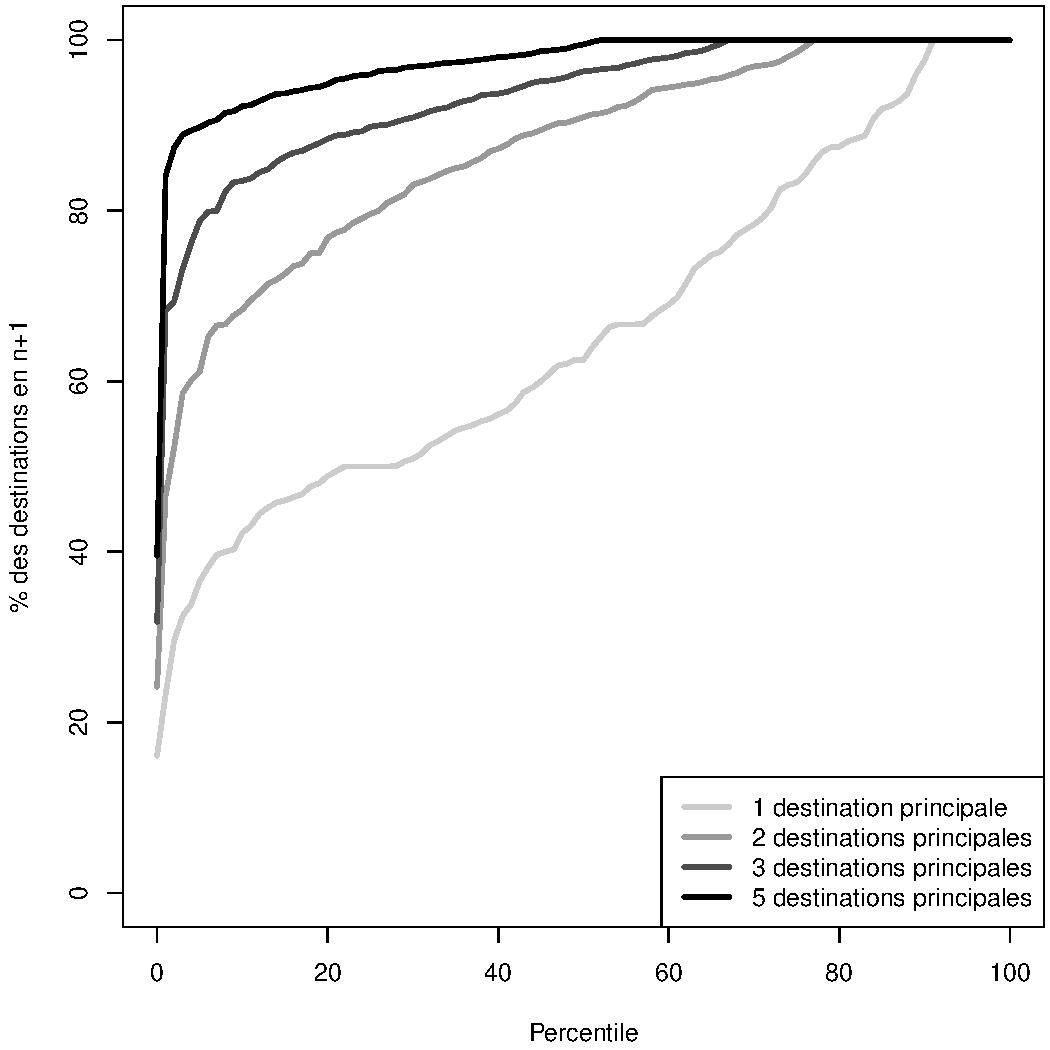
\includegraphics[width=0.5\linewidth]{pct.pdf}
\vspace{0.1cm}  
\begin{minipage}{12cm}%
\small \textsc{Lecture:} Pour environ 50 \% des grades, les 5 destinations les plus fréquentes représentent 100 \% des transitions observées.  
 \end{minipage}%
\end{figure}

En se concentrant sur les grades les plus représentés\footnote{TTH1 adjoint technique de 2eme classe, TAJ1 adjoint administratif de 2ème classe, 3001 aide soignant classe normale, 2432 infirmier de classe normale.}
pour les générations 1970-1979, il apparaît (voir la table 2) que l'écrasante majorité des transitions se fait dans le garde immédiatement supérieur quand elles ne se font pas vers un non-grade.
\begin{table}[h!]
    \label{tab:destination}
    \centering
    \caption{Destinations en cas de changement de grade (avec grade vide)} 
    \begin{tabular}{llrr}
\toprule
initial & destination &  nombre & part \\
\midrule
        &      autres &   90946 & 68 \% \\
        &        TTH1 &   21439 & 16 \% \\
        &        3001 &   10797 &  8 \% \\
        &        TAJ1 &   10137 &  8 \% \\
   TTH1 &             &    8416 & 43 \% \\
   TTH1 &        TTH2 &    8231 & 42 \% \\
   TTH1 &      autres &    2490 & 13 \% \\
   TTH1 &        TMD1 &     431 &  2 \% \\
   3001 &             &    5900 & 47 \% \\
   3001 &        3002 &    5389 & 43 \% \\
   3001 &      autres &     795 &  6 \% \\
   3001 &        2432 &     533 &  4 \% \\
   TAJ1 &        TAJ2 &    6346 & 48 \% \\
   TAJ1 &             &    5511 & 42 \% \\
   TAJ1 &      autres &     878 &  7 \% \\
   TAJ1 &        TAR1 &     396 &  3 \% \\
\bottomrule
\end{tabular}

\end{table}

En se limitant aux carrières ne présentant pas d'épisode ou la grade n'est pas renseigné, il apparaît que la destination est dans près de 80 \% des cas le grade immédiatement supérieur (passage à la classe supérieure) dans le corps ou le cadre d'emploi (voir la table 3).       

\begin{table}[h!]
    \label{tab:purged_destination}
    \centering
    \caption{Destinations en cas de changement de grade (carrières sans grade vide)} 
    \begin{tabular}{llrr}
\toprule
initial & destination &  nombre & part \\
\midrule
   TTH1 &        TTH2 &    7479 & 75 \% \\
   TTH1 &      autres &    1736 & 17 \% \\
   TTH1 &        TMD1 &     383 &  4 \% \\
   TTH1 &        TAJ1 &     362 &  4 \% \\
   3001 &        3002 &    5207 & 82 \% \\
   3001 &        2432 &     510 &  8 \% \\
   3001 &      autres &     505 &  8 \% \\
   3001 &        3121 &     134 &  2 \% \\
   TAJ1 &        TAJ2 &    5581 & 84 \% \\
   TAJ1 &      autres &     446 &  7 \% \\
   TAJ1 &        TAR1 &     345 &  5 \% \\
   TAJ1 &        TTH1 &     278 &  4 \% \\
   2432 &        2753 &    2645 & 79 \% \\
   2432 &      autres &     416 & 12 \% \\
   2432 &        2801 &     188 &  6 \% \\
   2432 &        1801 &      82 &  2 \% \\
\bottomrule
\end{tabular}

\end{table}

L'examen des transitions vers des grades plus élevés révèle une dynamique similaire (table 4).
\begin{table}[htbp]
    \label{tab:purged_second_destination}
    \centering
    \caption{Destinations en cas de changement de grade (carrières sans grade vide)} 
    \begin{tabular}{llrr}
\toprule
initial & destination &  nombre & part \\
\midrule
   TAJ2 &        TAJ3 &    5643 & 81 \% \\
   TAJ2 &        TAR1 &     882 & 13 \% \\
   TAJ2 &      autres &     351 &  5 \% \\
   TAJ2 &        TAJ1 &     109 &  2 \% \\
   TTH2 &        TTH3 &   10984 & 87 \% \\
   TTH2 &        TTM1 &     834 &  7 \% \\
   TTH2 &      autres &     613 &  5 \% \\
   TTH2 &        TTA2 &     169 &  1 \% \\
\bottomrule
\end{tabular}

\end{table}

Questions à discuter:
\begin{itemize}[leftmargin=1cm, parsep=0cm, itemsep=0cm, topsep=0cm] 
    \item Quel est le statut des transitions vers les états sans grade ? Est-ce un problème de données ou des mises en disponibilités et/ou des sorties de la FP? Doit-on gérer cela au niveau du module rémunération, carrière ou affiliation? 
\end{itemize}



%%%%%%%%%%%%%%%%%%%%%%%%%%%%%%%%%%%%%%%%%%%%%%%%%%%%%%%%%%%%%%%%%%%%%%%%%%%%

\ifx\isEmbedded\undefined
\newpage
\bibliographystyle{../../Divers/myagsm} 
\bibliography{../../Divers/biblio_these}
\end{document}
\else \fi

